% This LaTeX document needs to be compiled with XeLaTeX.
\documentclass[10pt]{article}
\usepackage[utf8]{inputenc}
\usepackage{amsmath}
\usepackage{amsfonts}
\usepackage{amssymb}
\usepackage[version=4]{mhchem}
\usepackage{stmaryrd}
\usepackage{graphicx}
\usepackage[export]{adjustbox}
\graphicspath{ {./images/} }
\usepackage[fallback]{xeCJK}
\usepackage{polyglossia}
\usepackage{fontspec}
\usepackage{newunicodechar}
\IfFontExistsTF{Noto Serif CJK TC}
{\setCJKmainfont{Noto Serif CJK TC}}
{\IfFontExistsTF{STSong}
  {\setCJKmainfont{STSong}}
  {\IfFontExistsTF{Droid Sans Fallback}
    {\setCJKmainfont{Droid Sans Fallback}}
    {\setCJKmainfont{SimSun}}
}}

\setmainlanguage{english}
\IfFontExistsTF{CMU Serif}
{\setmainfont{CMU Serif}}
{\IfFontExistsTF{DejaVu Sans}
  {\setmainfont{DejaVu Sans}}
  {\setmainfont{Georgia}}
}

\newunicodechar{⇒}{\ifmmode\Rightarrow\else{$\Rightarrow$}\fi}

\begin{document}
To utilize FOC we also need to argue that $V(k)$ is concave\\
Result 2: $V(k)$ is strictly concave if

\begin{itemize}
  \item $\Gamma(k)$ - convex
  \item $F\left(k, k^{\prime}\right)$-strictly concave
\end{itemize}

Proof: Use the same recursive approach\\
Suppose that $V_{0}$ is weakly concare:

$$
V_{0}\left(\lambda k_{1}+(1-\lambda) k_{2}\right) \geq \lambda V_{0}\left(k_{1}\right)+(1-\lambda) V_{0}\left(k_{2}\right)
$$

Show that $T V_{0}$ is strictly concare:

$$
\left(T V_{0}\right)\left(\lambda k_{1}+(1-\lambda) k_{2}\right)>\lambda\left(T V_{0}\right)\left(k_{1}\right)+(1-\lambda)\left(T V_{0}\right)\left(k_{2}\right), k_{1} \neq k_{2}
$$

Denote by $g(k)$ the optimal $k^{\prime}(k)$ associated with $V_{0}$\\
Then


\begin{align*}
& \lambda\left(T V_{0}\right)\left(k_{1}\right)+(1-\lambda)\left(T V_{0}\right)\left(k_{2}\right)= \\
& =\lambda F\left(k_{1}, g\left(k_{1}\right)\right)+\lambda \beta V\left(g\left(k_{1}\right)\right)+(1-\lambda) F\left(k_{2}, g\left(k_{2}\right)\right)+(1-\lambda) \beta V\left(g\left(k_{2}\right)\right) \\
& <\mid F-\text { strictg concare, } V \text {-concourc/ } \\
& <F\left(\lambda k_{1}+(1-\lambda) k_{2}, \lambda g\left(k_{1}\right)+(1-\lambda) g\left(k_{2}\right)\right)+\beta V\left(\lambda g\left(k_{1}\right)+(1-\lambda) g\left(k_{2}\right)\right) \\
& \leq \mid \text { if } \lambda g\left(k_{1}\right)+(1-\lambda) g\left(k_{2}\right) \in \Gamma\left(\lambda k_{1}+(1-\lambda) k_{2}\right) \mid \\
& \leq T V_{0}\left(\lambda k_{1}+(1-\lambda) k_{2}\right) \tag{x}
\end{align*}


\section*{When does (*) hold?}
$$
\begin{aligned}
& \Gamma(k) \text { - convex } \\
& \text { corresponderce }
\end{aligned} \Rightarrow \operatorname{\lambda g(k_{1})+(1-\lambda )g(k_{2})\in \Gamma (\lambda k_{1}+(1-\lambda )k_{2})} 1 \text { since } g\left(k_{1}\right) \in \Gamma\left(k_{1}\right), g\left(k_{2}\right) \in \Gamma\left(k_{2}\right)
$$

Example: $\Gamma(k)=\left\{k^{\prime}: 0 \leq k^{\prime} \leq f(k)\right\}$

$$
\left.\begin{array}{c}
k_{1}^{\prime} \leq f\left(k_{1}\right) \\
k_{2}^{\prime} \leq f\left(k_{2}\right) \\
\Gamma
\end{array}\right] \Rightarrow \begin{gathered}
\lambda k_{1}^{\prime}+(1-\lambda) k_{2}^{\prime} \leq \lambda f\left(k_{1}^{\prime}\right)+(1-\lambda) f\left(k_{2}^{\prime}\right) \leq \\
\leq(f-\text { concare }) \leq f\left(\lambda k_{1}^{\prime}+|1-\lambda| k_{2}^{\prime}\right)
\end{gathered}
$$

( $\left.k_{2}^{\prime} \leq f \mid k_{2}^{\prime}\right) \mid \Rightarrow \leq(f$-concave $) \leq f\left(\lambda k_{1}^{\prime}+|1-\lambda| k_{2}^{\prime}\right)$ Thus $\Gamma(k)$ is convex is $f$-concave\\
$\Rightarrow T V_{0}$ is strictly concave $\Rightarrow / \lim _{n \rightarrow \infty}$, apply Tence more/ $\Rightarrow V(k)$ is strictly concare.

Gen be verified that $u(\cdot), f()$ satisfy the desised properties if $u(\cdot)$-strictlyconcave, ince.\\
$f\left({ }^{\prime}\right)$ - concave

Remark: Such recursive approach is very useful for charyacterizmy $V(k)$ :

\begin{itemize}
  \item differentiability
  \item bounds
  \item comparative statics (how does V(.) change if a parameter changes).
\end{itemize}

\section*{Using the properties of the value function:}
If the solution to (BE) is interior ⇒ it satisfies FOC:\\
( $\left.k^{\prime}\right): \quad F_{2}\left(k, k^{\prime}\right)+\beta V^{\prime}\left(k^{\prime}\right)=0$\\
Or interms of $U($.$) and fla)$

$$
u^{\prime}\left(f(k)-k^{\prime}\right)=\beta V^{\prime}\left(k^{\prime}\right)
$$

current cost $=$ future benefit\\
Cinterms of marginal (interms of discountal utility, future value)\\
Devote by $g(k)$ the optimal $k^{\prime}$\\
What can we soy about its properties?\\
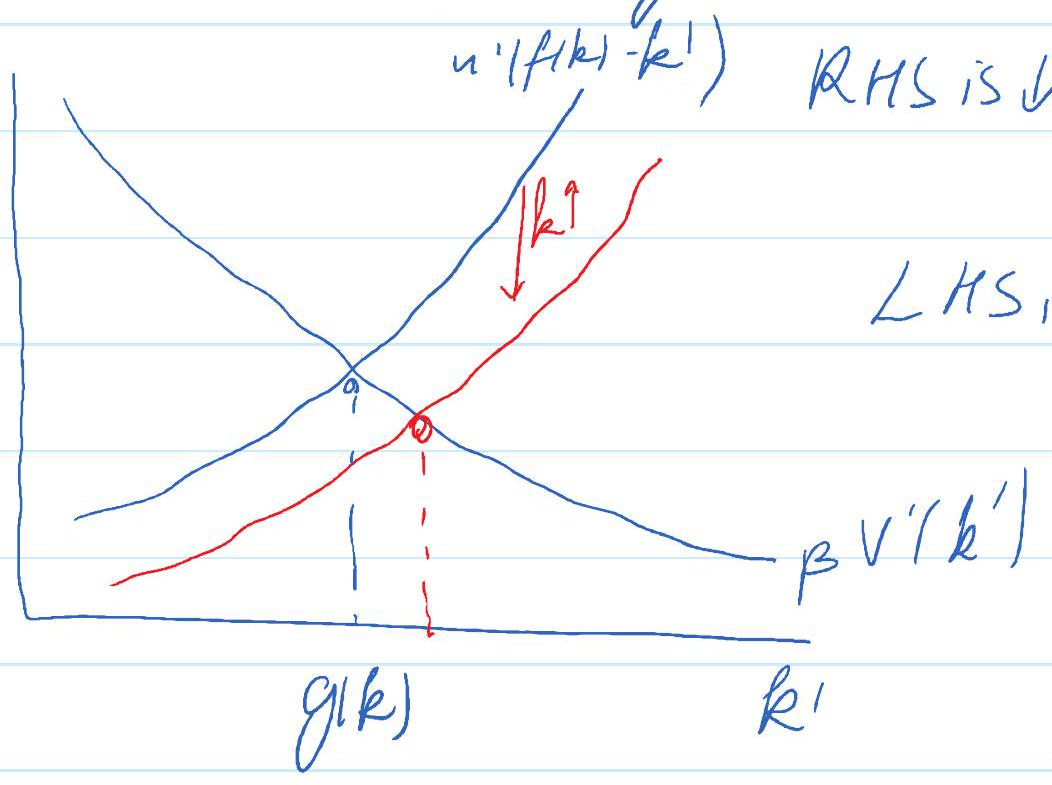
\includegraphics[max width=\textwidth, alt={}, center]{08cefc7c-c55b-49d2-b784-31419080f64d-3_785_1052_1598_416}

$$
R H S \text { is } \psi \text { since } V(k) \text { is }
$$

concowe!

LHS is $T$ since $u(c)$ isconcoule\\
$k \uparrow \Rightarrow f(k) \hat{\uparrow} \Rightarrow \mid u\left(c \mid\right.$-concave $\left.\mid \Rightarrow u^{\prime}(\mid t k) k^{\prime}\right) \downarrow$

$$
\begin{aligned}
& k 1 \Rightarrow f(k) 1, \mid u(c) \text {-concover } \Rightarrow u(r(k)-k) v \\
& \Rightarrow g(k) \text { is } T \text { in } k
\end{aligned}
$$

Thus, concervity of $V(k)$ and $n(c)$ implics that $g(k)$ is increasing\\
Isave nore if there is more capital today)

Euler Equation -- once again!

$$
V(k)=\max _{k^{\prime} \in \Gamma(k)}\left\{F\left(k, k^{\prime}\right)+\beta V\left(k^{\prime}\right)\right\}
$$

If the solution is interior ⇒

$$
\left.(F O C): \quad F_{2}\left(k, k^{\prime}\right)+\beta v^{\prime}\left(k^{\prime}\right)=0 \quad \Rightarrow \quad k^{\prime}=g^{\prime} k\right)
$$

Envelope condition:

$$
\begin{aligned}
V(k) & =F(k, g(k))+\beta V(g(k)) \\
\Rightarrow V^{\prime}(k) & =F_{1}(k, g(k))+\underbrace{\left[F_{2}(k, g(k))+\beta V^{\prime}(g(k))\right] g^{\prime}(k)}_{=0 \text { by } F O C} \\
\Rightarrow V^{\prime}(k) & =F_{1}(k, g(k)) \quad(E C) \text { envelope condition }
\end{aligned}
$$


\begin{equation*}
(F O C+E C) \Rightarrow \quad F_{2}(k, g(k))+\beta F_{1}(g(k), g(g(k)))=0 \tag{EE}
\end{equation*}


familiar Euler Equation!!! "\\
Or reevrite it in terms of U(.) and $f(-)$ :\\
$\left.u^{\prime}(f(k)-g(k))=\beta c^{\prime}(H g(k))-g(g(k))\right) \cdot f^{\prime}(g(k))$\\
Formally, this is a functional equation w, the respect to $g(k)$ 。

If a closed-form solution exists, it of course can be found wsing the guess and.\\
verify nothod (guess $g(k)$, find coefficients) However, (EE) does not hold if the solution socrear solution

Or if the closed-form solution choes not exits, (EE) might be hard to solve nemerically: there is no "convergence" result like for $V(k)$ in the (BE) (contraction mapping)

Technickally, ane can pewrite (EE):

$$
g(k)=\underbrace{\left.f(k)-\left(u^{\prime}\right)^{-1}\left(\beta u^{\prime}(f(g / k))-g(g(k))\right) \cdot f^{\prime}(g(k))\right)}_{\text {operator on } g / k)}
$$

But it is messy, likely not a contraction (wr.t. write)

⇒ While (BE), is easy to solve numerically, (EE) may be tridey..


\end{document}